\documentclass{beamer}

\setlength{\unitlength}{1cm} 
\usetheme{Madrid}

\usepackage[utf8]{inputenc}

\usepackage{amsmath}
\usepackage{graphicx}

\newcommand{\norm}[1]{\left\lVert#1\right\rVert}

\title{How directed is a directed network?}
\subtitle{MacKay, Johnson, and Sansom}
\author{Andrea Titton}
\institute{Tinbergen Institute}
\date{04/12/2020}

\begin{document}

\frame{\titlepage}
\nocite{*}

\begin{frame}
    \frametitle{Trophic level}
    Measure of hierarchical structure among nodes
    \begin{columns}
        \begin{column}{.49\textwidth}
            \begin{figure}
                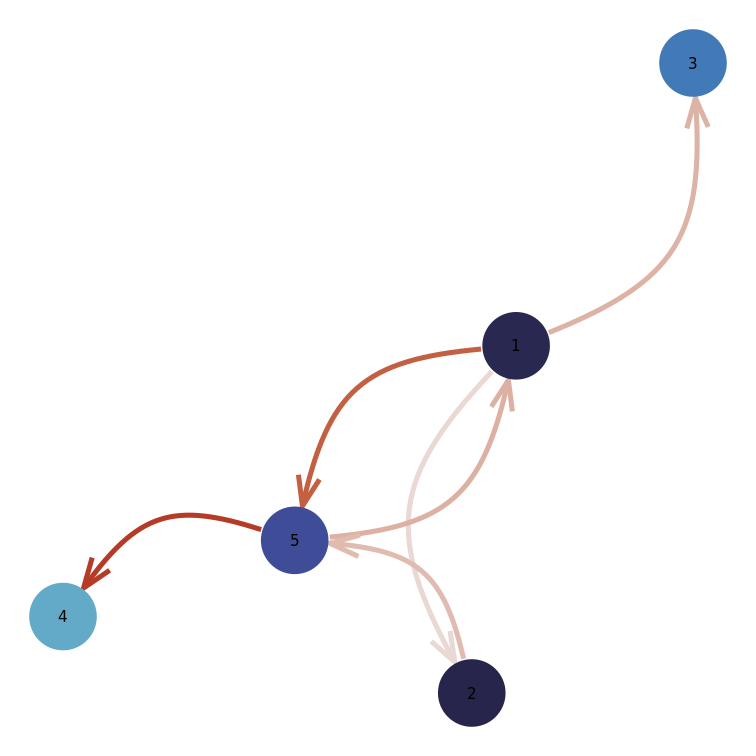
\includegraphics[width=0.8\linewidth,height=0.8\textheight,keepaspectratio]{../../plots/presentations/lv-network.png}
            \end{figure}
        \end{column}
        \begin{column}{.48\textwidth}
            The trophic level solves,
            $\Lambda h = v$ where
            $\Lambda = \underbrace{diag(u)}_{\textit{total weight}} - W - W^T$
            and $v$ is the imbalance.
            \hspace{2\unitlength}
            \begin{itemize}
                \item Ecologic stability
                \item Neural cascade
                \item Epidemics
            \end{itemize}
        \end{column}
    \end{columns}
\end{frame}

\begin{frame}
    \frametitle{Trophic incoherence}
    \begin{equation}
        F_0 = \frac{\sum_{mn} w_{mn} \cdot (h_n - h_m - 1)^2}{\sum_{mn} w_{mn}} \in [0, 1]
    \end{equation}
    \begin{columns}
        \begin{column}{.49\textwidth}
            \begin{figure}
                \textbf{$F_0 = 1$}\par\medskip
                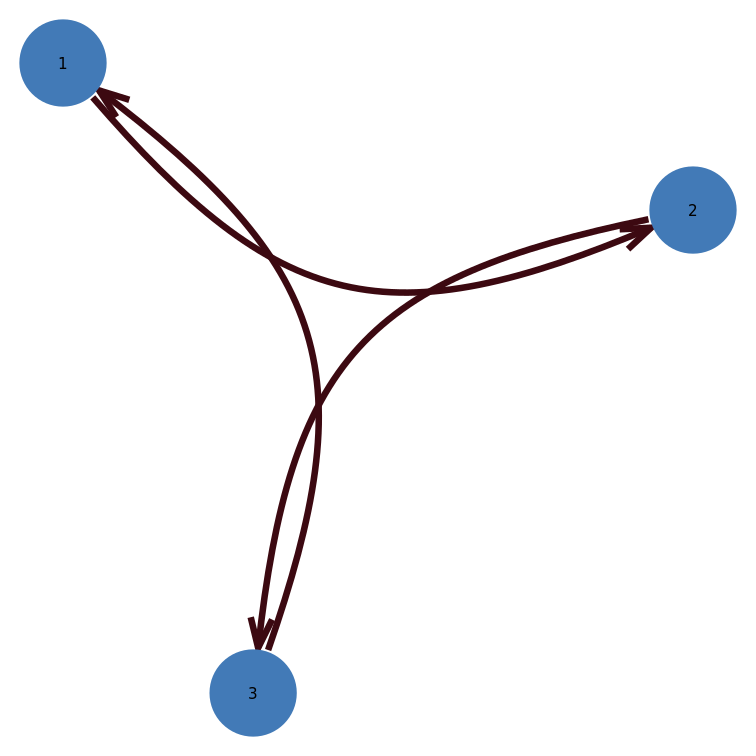
\includegraphics[width=0.8\linewidth,height=0.8\textheight,keepaspectratio]{../../plots/presentations/lv-network-coherent.png}
            \end{figure}
        \end{column}
        \begin{column}{.49\textwidth}
            \begin{figure}
                \textbf{$F_0 = 0$}\par\medskip
                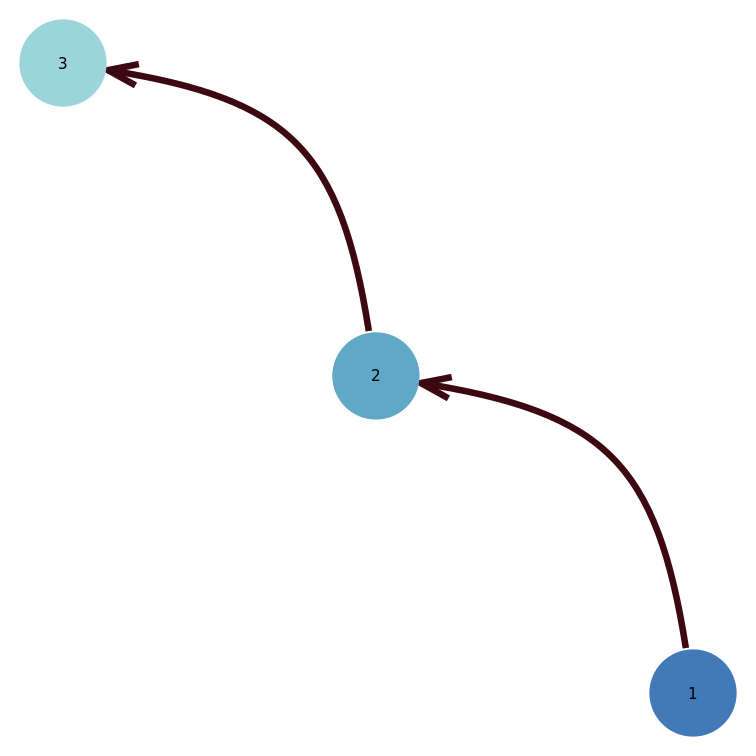
\includegraphics[width=0.8\linewidth,height=0.8\textheight,keepaspectratio]{../../plots/presentations/lv-network-incoherent.png}
            \end{figure}
        \end{column}
    \end{columns}
\end{frame}

\begin{frame}
    \frametitle{Empirical ``Why" - 1}
    \begin{columns}
        \begin{column}{.49\textwidth}
            Relative notions are ``old" trophic level in ecology
            and upstreamness in economics.
            \begin{itemize}
                \item Does not require basal/terminal nodes (which lead to biases)
                \item Robust to cycles
                \item Present a ``maximum" coherence
            \end{itemize}
        \end{column}
        \begin{column}{.49\textwidth}
            \begin{figure}
                \textbf{$F_0 = 0.76$}\par\medskip
                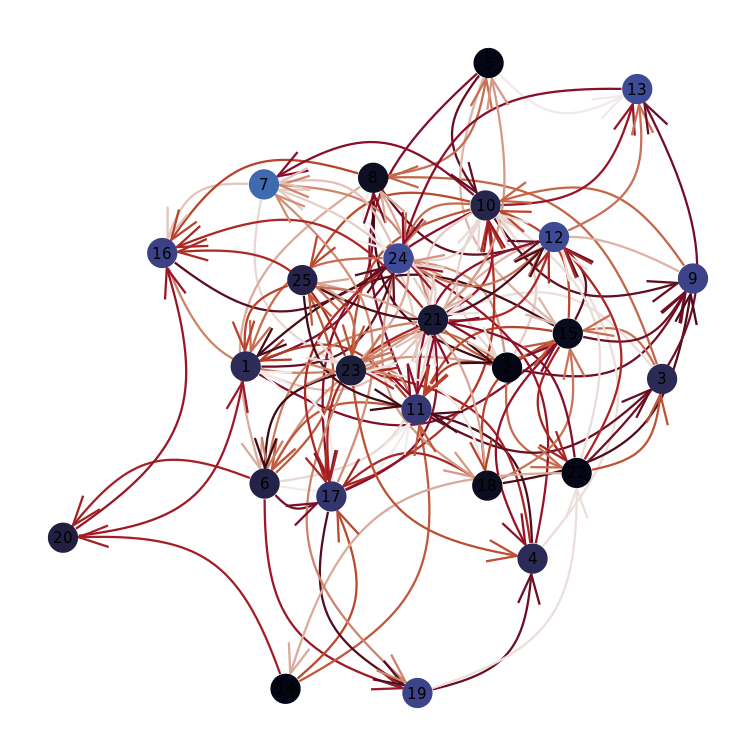
\includegraphics[width=\linewidth,height=\textheight,keepaspectratio]{../../plots/presentations/lv-network-big.png}
            \end{figure}
        \end{column}
    \end{columns}
\end{frame}

\begin{frame}
    \frametitle{Empirical ``Why" - 2}
    \begin{columns}
        \begin{column}{.3\textwidth}
            \begin{itemize}
                \item Comparable among different graphs (i.e. different countries IOs)
                \item Results hold on partial graphs
            \end{itemize}
        \end{column}
        \begin{column}{.69\textwidth}
            \begin{figure}
                \includegraphics[width=\linewidth,height=\textheight,keepaspectratio]{../graphs/sectors-mackay.png}
            \end{figure}
        \end{column}
    \end{columns}
\end{frame}

\begin{frame}
    \frametitle{Theoretical ``Why"}
    Consider the simple model (without loss of generality),
    \begin{equation*}
        x_n^\prime =\frac{1}{r} \sum_{m} x_m\cdot w_{m, n}
    \end{equation*}

    It can be shown that,

    \begin{equation*}
        \lim_{t \xrightarrow{} \infty} t^{-1} \log \norm{x(t)} \approx\frac{1}{2} \cdot \left( 1 - \frac{1}{F_0}\right) + log \norm{W} - log(r)
    \end{equation*}

    Hence,

    \begin{equation}
        \exp\left(\frac{1}{2} \left( 1 - \frac{1}{F_0}\right) \right) \cdot \norm{W} < r \implies \norm{x} \xrightarrow{t\xrightarrow{} \infty} 0
    \end{equation}

\end{frame}

\begin{frame}
    Back to our first example,
    \begin{figure}
        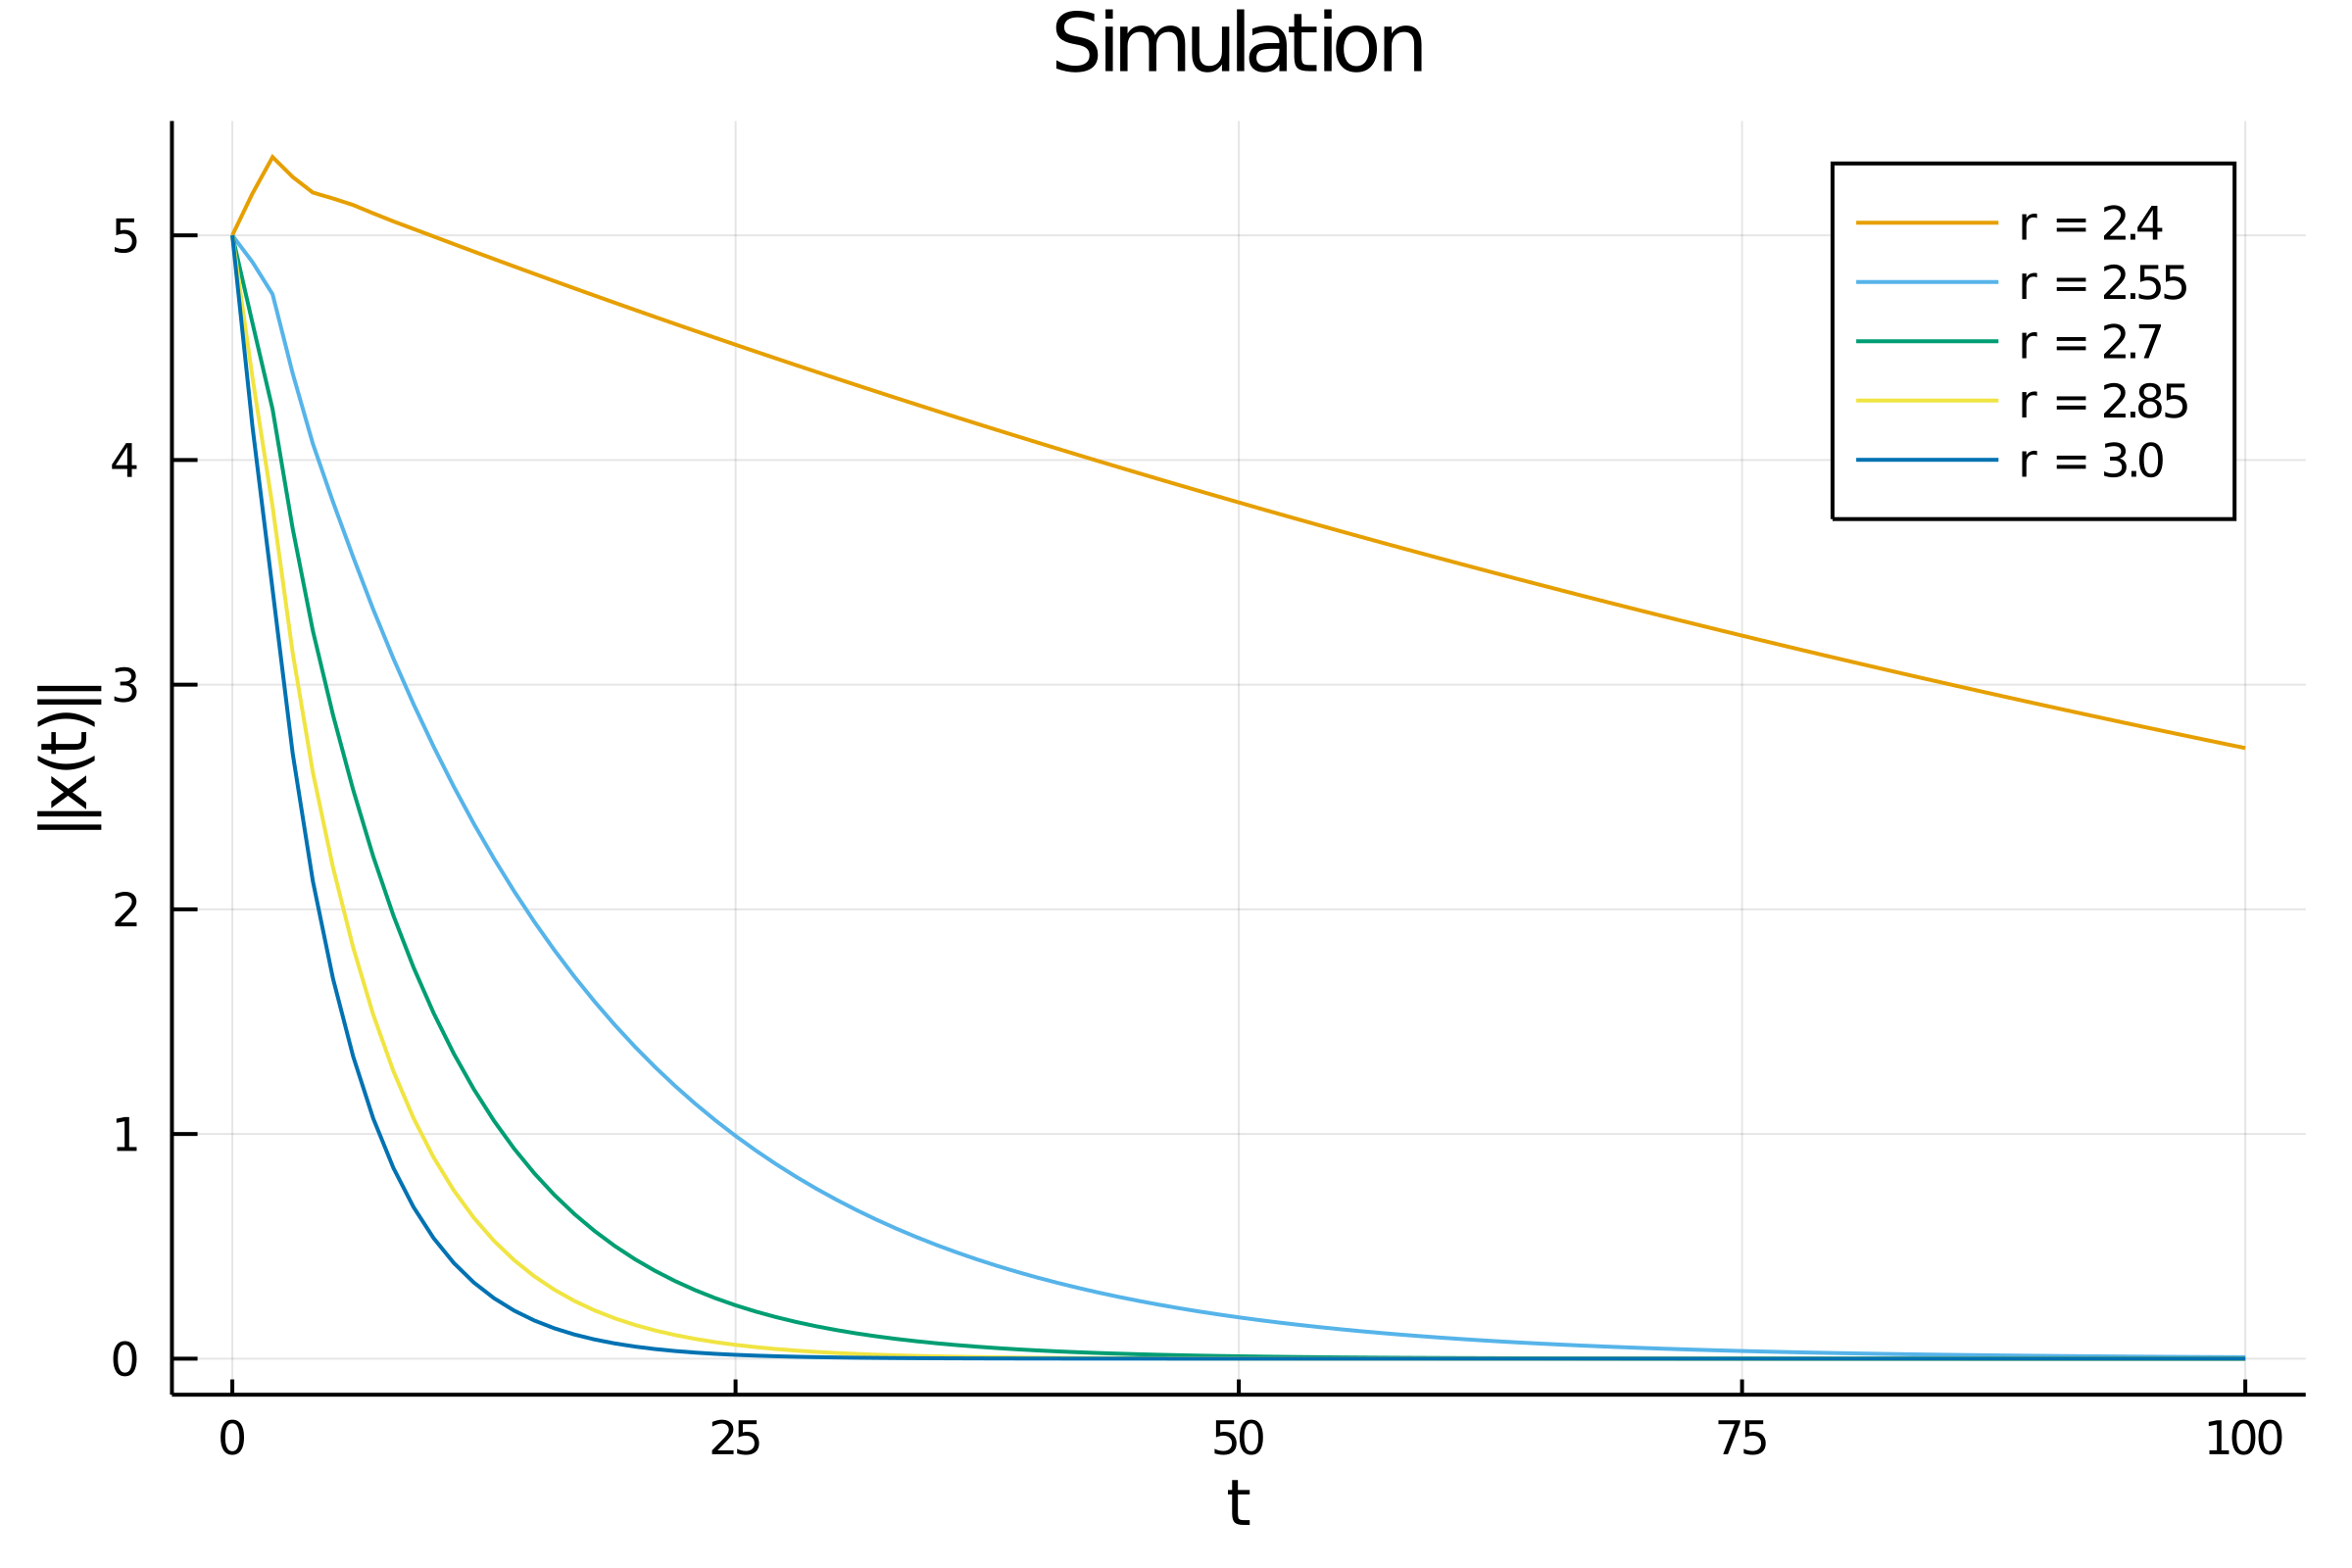
\includegraphics[width=\linewidth,height=\textheight,keepaspectratio]{../../plots/presentations/dynamics.png}
    \end{figure}
\end{frame}


\begin{frame}
    \frametitle{Research proposal}
    Using trophic coherence to study the resilience of electricity networks. Agents are prosumers and make decision in discrete time.


    \begin{columns}
        \begin{column}{.49\textwidth}
            Electricity market, with $W(x(t))$ and $F_t$, that maximizes resilience, while being
            \begin{itemize}
                \item Diffused
                \item With heterogenous agents
                \item Hit by climate shocks
            \end{itemize}
        \end{column}
        \begin{column}{.49\textwidth}
            \begin{figure}
                \textbf{$F_0 = 0.70$}\par\medskip
                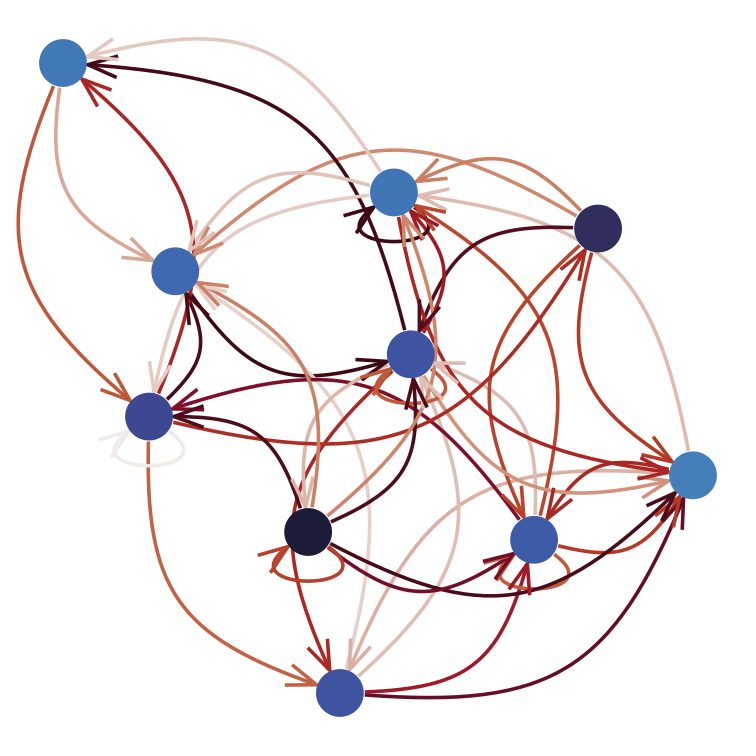
\includegraphics[width=\linewidth,height=0.4\textheight,keepaspectratio]{../../plots/presentations/electricity.png}
            \end{figure}
        \end{column}
    \end{columns}
\end{frame}


\begin{frame}[allowframebreaks]{Bibliography}
    \bibliographystyle{apa}
    \bibliography{refs.bib}
\end{frame}

\end{document}